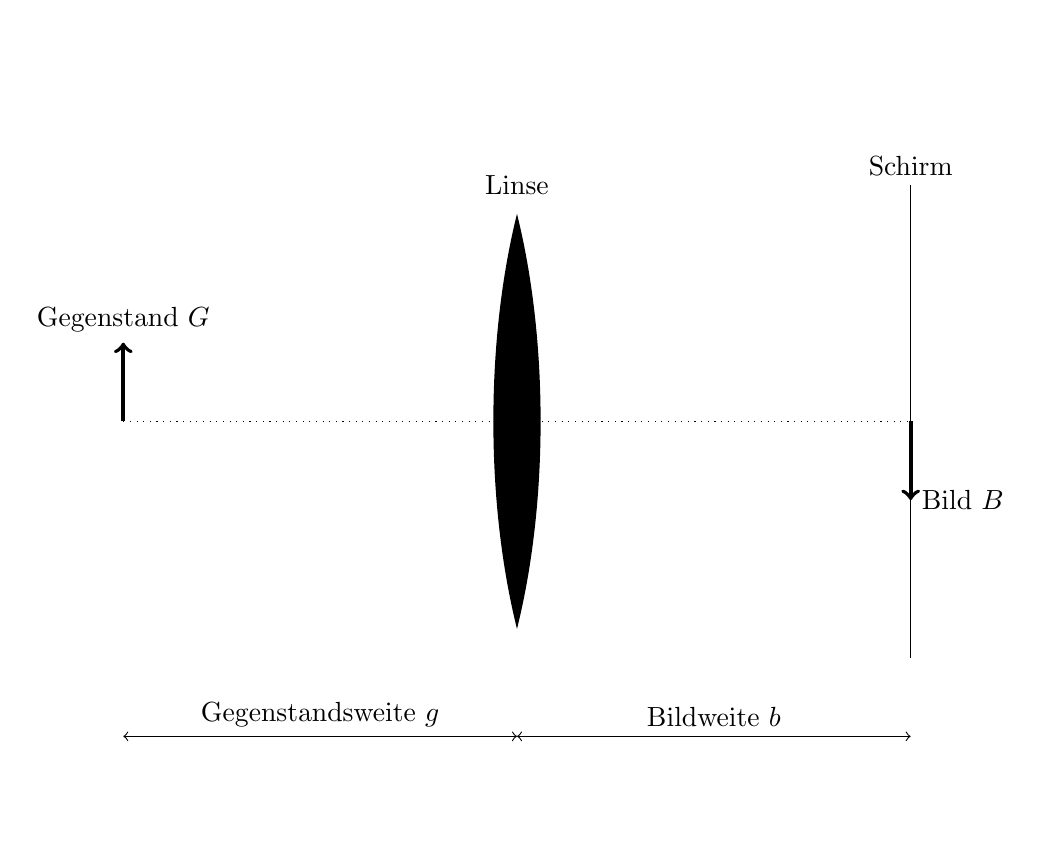
\begin{tikzpicture}

%Mittellinie
\draw [dotted] (-5,0)--(5,0);

%Gegenstand
\draw [->=latex, line width=0.05cm] (-5,0)--(-5,1) node [above] {Gegenstand $G$};
%Bild
\draw [->=latex, line width=0.05cm] (5,0)--(5,-1) node [right] {Bild $B$};

\begin{scope}[xscale=2, yscale=5]
\clip (-0.85,0) circle (1cm);
\clip (0.85,0) circle (1cm);
\fill(-2,-2) rectangle (2,2);
\end{scope}

\draw (0,3) node {Linse};

%Schirm
\draw (5,-3)--(5,3) node [above] {Schirm};


\draw [<->=latex] (-5,-4)--(0,-4) node [midway, above] {Gegenstandsweite $g$};
\draw [<->=latex] (0,-4)--(5,-4) node [midway, above] {Bildweite $b$};
\end{tikzpicture}